%!TEX root = bachelor.tex
\chapter{Methodik}
\label{ch:method}
In diesem Kapitel werden zwei Verfahren zur Entzerrung von Kegeloberflächen vorgestellt.
Zunächst gehen wird auf das verwendete Kalibrierungsmuster eingegangen, worauf hin die einzelnen Schritte der Entzerrung erläutert werden.

Die geometrischen Eigenschaften des Kegelstumpfs $(r, R, \Delta H)$ können gemessen und somit als bekannt angenommen werden.
Darüber hinaus wird angenommen, dass sich das Zentrum des Deckkreises an der Position $(0,0,0)$, sowie das Zentrum des Grundkreises an der Position $(0,\Delta H, 0)$ im Weltkoordinatensystem befindet (siehe Abbildung \ref{fig:coneFrustum} in Kapitel \ref{s:cone}). Durch diese Einschränkung gehen jegliche absolute Größenverhältnisse verloren. Die Larven können jedoch weiterhin relativ zu einander verglichen werden.


\section{Kalibrierungsmuster}
\label{s:calibrationPattern}
Um eine Beziehung zwischen Bildpunkten und Kegelpunkten herstellen zu können, ist ein Kalibrierungsmuster notwendig.

Die Wahl des Kalibrierungsmusters spielt dabei eine entscheidende Rolle bei der Robustheit und Präzision der Entfaltung. Es muss gewährleistet sein, dass die charakteristischen Merkmale des Musters auch bei leichten Abweichungen der Kamera vom Lot und schlechteren Beleuchtungssituationen zuverlässig erkannt werden. Das Muster muss darüber hinaus so entworfen sein, dass beim Zusammenlegen im Kegel, dessen geometrische Eigenschaften nicht verfälscht, sondern realitätsgetreu wiedergeben werden.

\subsection{Aufbau des Kalibrierungsmusters}
Die Wahl fiel auf ein Muster, dass in äquidistanten Abständen $\Delta R$, beginnend mit dem Radius $r$ des Deckkreises (siehe Abbildung \ref{fig:coneFrustum}) Kreislinien und in gleichen Winkelabständen $\Delta \alpha$ auf der Seitenhöhe Liniensegmente besitzt. Das zusammengelegte Muster ist in Abbildung \ref{fig:calibrationPatternTop} skizziert, beziehungsweise das entfaltete in Abbildung \ref{fig:calibrationPattern}. Die Anzahl der Kreislinien wird mit $n$ gekennzeichnet, die Anzahl sichtbarer Liniensegmente im Kegel mit $m$. Zu beachten ist, dass bedingt durch das Entfalten, in Abbildung \ref{fig:calibrationPattern}  ein Liniensegment doppelt zu sehen ist. Die schwarzen Kreise werden als Samples bezeichnet.

Dadurch dass die Geometrie des Kegels bekannt ist, kann jedem Sample ein Punkt auf dem Kegel im Weltkoordinatensystem zugeordnet werden. Da ein Kegel beliebig um die $y$-Achse rotiert werden kann, ist diese Zuordnung zunächst nicht eindeutig. Dazu sei angenommen, dass das Liniensegment mit dem kleinsten Winkel zur $x$-Achse mit dem Kegelwinkel $\theta = 0$ korrespondiert (siehe Gleichung \ref{eq:paramFrustum} in Kapitel \ref{s:cone}).

\begin{figure}[!htb]
	\centering
	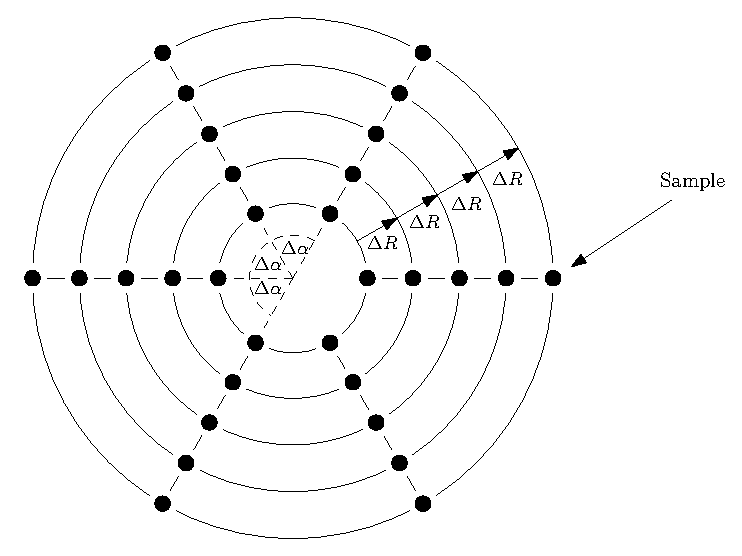
\includegraphics[scale=.8]{images/calibrationPatternTop.eps}
	\caption{Kalibrierungsmuster von oben mit $n = 5, m = 6$}
	\label{fig:calibrationPatternTop}
\end{figure}


\begin{figure}[!htb]
	\centering
	\includegraphics[scale=.7]{images/calibrationPattern2.eps}
	\caption{Kalibrierungsmuster entfaltet mit $n = 5, m = 6$}
	\label{fig:calibrationPattern}
\end{figure}

Zur Konstruktion des Musters benötigt man $\Delta S$ und $s$, die man aus der Geometrie des Kegels errechnen kann und außerdem den Öffnungswinkel, der gegeben ist als $\alpha = 2\pi\frac{R}{S}$ (siehe Gleichung \ref{eq:paramLateral} in Kapitel \ref{s:cone}).

\subsection{Anzahl der Samples}
Die Anzahl der Samples sollte groß genug sein, um möglichst viele geometrische Informationen des Kegels zu erhalten, aber klein genug, dass eine Detektion der Samples problemlos möglich ist. Insbesondere auf dem innersten Kreis, macht sich eine zu hohe Sampleanzahl negativ bemerkbar, da der Abstand der Samples zueinander sehr klein wird, was eine Detektion erschwert. Des Weiteren sollte noch ein möglichst großer Teil der Kreislinien zu sehen bleiben, da diese für die spätere Ellipsendetektion benötigt werden.


\section{Intrinsische Kamerakalibrierung}
\label{s:intrinsic}
Bedingt durch die Wahl einer Weitwinkelkamera, sind die Bilder von einer starken tonnenförmigen (nach außen gewölbte) Verzerrung geprägt, wie in Abbildung \ref{fig:calib} zu sehen. Diese muss herausgerechnet werden, da sonst Abstände im Bild nicht mehr der Realität entsprechen und dadurch die Präzision der Entfaltung stark abnimmt (siehe Kapitel \ref{ch:analysis}). Es wird also im ersten Schritt eine Kamerakalibrierung durchgeführt.


\begin{figure}[!htb]
	\centering
\begin{subfigure}{.5\textwidth}
	\centering
	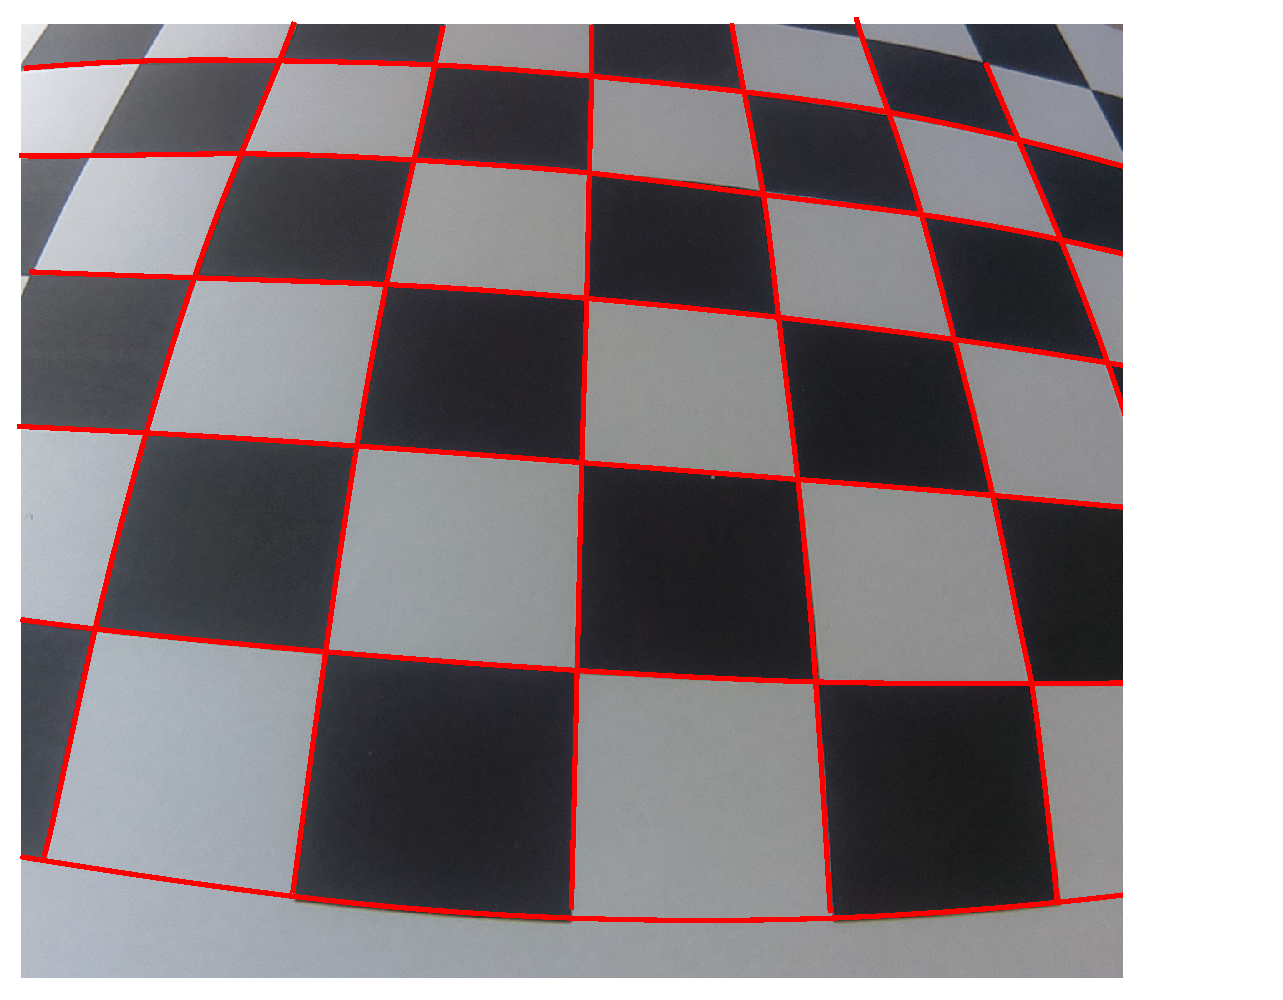
\includegraphics[scale=.35]{images/calibrationRaspi.eps}
	\caption{vor Kalibrierung}
	\label{fig:calibDist}
\end{subfigure}%
\begin{subfigure}{.5\textwidth}
	\centering
	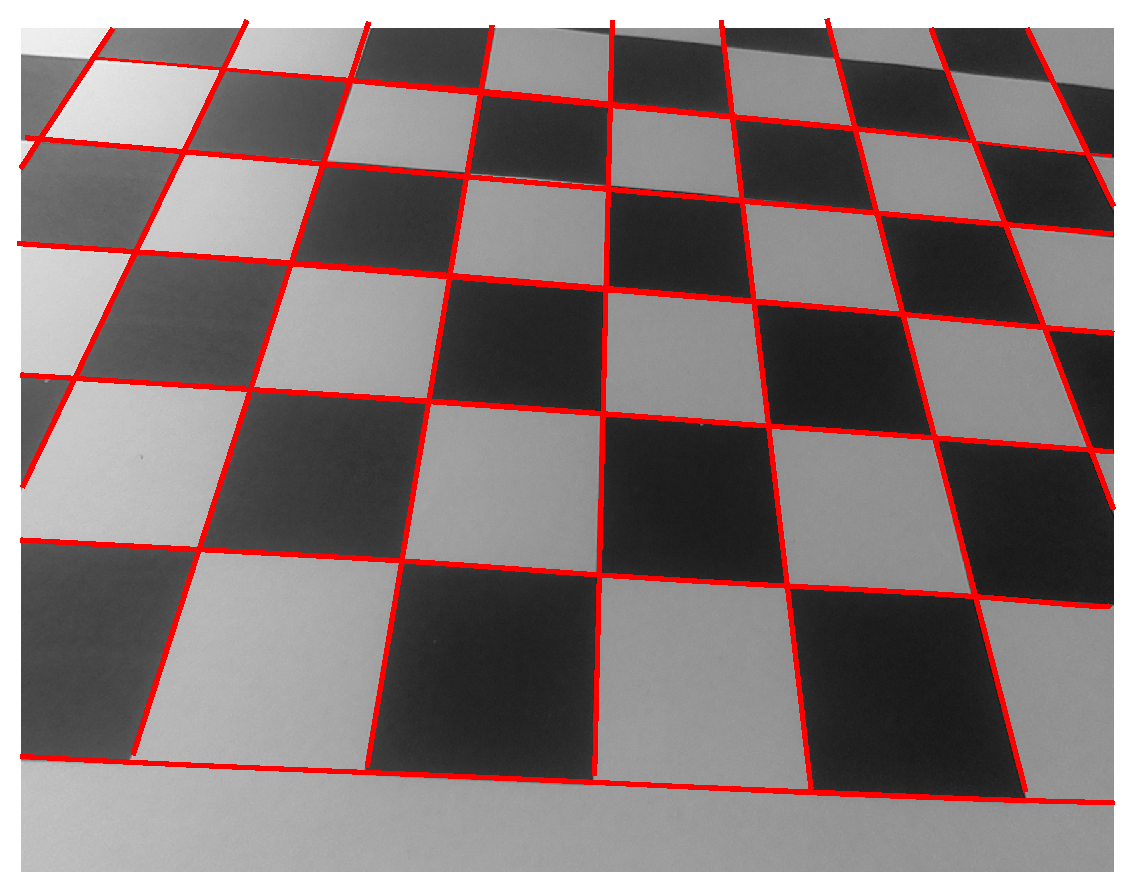
\includegraphics[scale=.4]{images/calibrationRaspi2.eps}
	\caption{nach Kalibrierung und Entzerrung}
	\label{fig:calibUndist}
\end{subfigure}
\caption{Kamerakalibrierung}
\label{fig:calib}
\end{figure}

\section{Detektion der charakteristischen Punkte}

Nach der Kamerakalibrierung und entsprechender Entzerrung werden die Bildkoordinaten der Samples bestimmt. Dazu wird ein Blob-Detektor (siehe Kapitel \ref{s:blob}) benutzt.
Um ein Sample korrekt detektieren zu können, muss sich der Punkt farblich stark von seiner Umgebung abheben (siehe Definition eines Blobs \ref{def:blob}). Das bedeutet, dass ein Sample freigestellt (helle homogene Umgebung) sein muss. Insbesondere dürfen die Kreislinien und Liniensegmente des Kalibrierungsmusters also nicht durchgezogen sein.

Nach der Detektion werden die Blobs nach folgenden Kriterien gefiltert:

\begin{itemize}
	\item \textbf{Fläche:} zu kleine Blobs werden verworfen
	\item \textbf{Rundheit:} zu unrunde Blobs werden verworfen. Rundheit ist hier definiert als $circ = \frac{4\pi\cdot \textrm{Fläche}}{\left(\textrm{Umfang}\right)^2}\in[0,1]$, wobei ein Kreis mit $circ = 1$ maximal rund ist.
	\item  \textbf{Konvexität:} zu unkonvexe Blobs werden verworfen. Konvextität ist hier definiert \\als $conv = \frac{\textrm{Fläche Blob}}{\textrm{Fläche konvexe Hülle}}$
\end{itemize}

In Abbildung \ref{fig:blobDetect} ist beispielhaft links ein Grauwertbild und rechts die detektierten Blobs (rot) auf dem gleichen Bild nach der Kameraentzerrung zu sehen.


\begin{figure}[!htb]
	\centering
	\begin{subfigure}{.5\textwidth}
		\centering
		\includegraphics[width=.9\textwidth]{images/coneRasp.jpg}
		\caption{Grauwertbild}
	\end{subfigure}%
	\begin{subfigure}{.5\textwidth}
		\centering
		\includegraphics[width=.9\textwidth]{images/coneRaspDetectedDots.png}
		\caption{Grauwertbild und detektierte Blobs (rot)}
	\end{subfigure}
	\caption{detektierte Samples}
	\label{fig:blobDetect}
\end{figure}


\section{Ellipsen-Detektion}
\label{s:ellipseDetection}

Nachdem die Sample-Positionen bestimmt wurden, muss für jeden Sample entschieden werden, auf welcher der Kreislinien es liegt. Da die Kreise, bedingt durch perspektivische Verzerrung, zu Ellipsen werden, wird ein Verfahren benötigt, dass Ellipsen erkennt.
Dies kann mit Hilfe von zwei verschiedenen Verfahren realisiert werden. Zunächst wird ein Ansatz zur Parameterschätzung der Ellipsen mittels RANSAC erläutert, woraufhin auf einen Ansatz eingegangen wird, bei dem die Ellipsen iterativ mit Hilfe von Deformable Templates
detektiert werden.

\subsection{RANSAC}


\begin{figure}[!htb]
	\centering
	\begin{subfigure}{.5\textwidth}
		\centering
		\includegraphics[width=.9\textwidth]{images/grey.png}
		\caption{Grauwertbild}
		\label{fig:beforeCanny}
	\end{subfigure}%
	\begin{subfigure}{.5\textwidth}
		\centering
		\includegraphics[width=.9\textwidth]{images/canny.png}
		\caption{Kantenbild}
		\label{fig:afterCanny}
	\end{subfigure}
	\caption{Canny-Kantendetektion}
	\label{fig:canny}
\end{figure}

Zunächst werden die Kanten mit Hilfe des Canny-Kantendektors \cite{Canny1986} erfasst (siehe Abbildung \ref{fig:canny}).
Anschließend wird eine möglichst genau Schätzung des Zentrum der innersten Ellipse vorgenommen.
Dafür wird Hough-Transformation (siehe Kapitel \ref{s:hough}) benutzt, um Linien im Kantenbild zu detektieren.
Es werden anschließend die Schnittpunkte aller Liniensegmente bestimmt.
Die Liniensegmente schneiden sich dabei genau dann in einem Punkt, wenn sich die Kamera genau im Lot befindet und perfekt auf das Zentrum des Deckkreises ausgerichtet ist.
Darüber hinaus werden, auf Grund der Liniendicke auf dem Kalibrierungsmuster, durch den Canny-Algorithmus viele Linien als doppelte Linien gekennzeichnet\footnote{Stellt man sich ein relativ breites Liniensegment vor, so gibt es einmal den Übergang vom Hintergrund auf die Linie, sowie den Übergang von der Linie wieder auf den Hintergrund}. Auch ein inhomogener Hintergrund, erschwert die Ermittlung eines Mittelpunkts. Befinden sich Objekte im Hintergrund, werden durch die Kantendetektion auch deren Kanten ermittelt. Die Hough-Transformation detektiert auch außerhalb des Kalibrierungsmusters Linien. Die Schnittpunkte mit solchen Linien können beliebig stark von dem eigentlichen Mittelpunkt abweichen. Würde man an dieser Stelle beispielsweise den Mittelwert aller Schnittpunkte (elementweise) berechnen, könnten solche Ausreißer die Lokalisierung des Mittelpunkts erheblich verschlechtern.

Um möglichst robust einen Kandidaten auszuwählen, wird der Median der $x$-Koordinaten der Schnittpunkte und der Median der $y$-Koordinaten bestimmt. Die erhaltenen Koordinaten bilden den Schnittpunkt, wie in Abbildung \ref{fig:houghLines} beispielhaft zu sehen.

\begin{figure}[!htb]
	\centering
	\includegraphics[scale=.25]{images/houghLines.png}
	\caption{Hough-Transformation zur Linien-Detektion (rot) und bestimmter Schnittpunkt (grün) }
	\label{fig:houghLines}
\end{figure}

Von diesem Schnittpunkt aus werden, in einer vorher definierten Anzahl, gleichmäßig, in alle Richtungen Strahlen ausgesendet.
Trifft ein Strahl ein Kantenpixel, wird dessen Position gekennzeichnet, trifft er den Rand des Bildes, wird er ignoriert. In Abbildung \ref{fig:rayCastWOE} sind beispielhaft die getroffenen Kantenpixel (weiß) und der zugehörige Aussendepunkt eingezeichnet.

\begin{figure}[!htb]
	\centering
	\begin{subfigure}{.5\textwidth}
		\centering
		\includegraphics[width=.9\textwidth]{images/rayCast0.png}
		\caption{bestimme Pixel-Positionen}
		\label{fig:rayCastWOE}
	\end{subfigure}%
	\begin{subfigure}{.5\textwidth}
		\centering
		\includegraphics[width=.9\textwidth]{images/rayCast0Ellipse.png}
		\caption{bestimme Ellipse (grün)}
		\label{fig:rayCastWE}
	\end{subfigure}
	\caption{Ellipsendetektion: bestimme Pixel-Positionen (weiß), Aussendepunkt (gelb)}
	\label{fig:rayCast}
\end{figure}

Mit Hilfe der Postionen der getroffenen Pixel, wird anschließend mittels RANSAC (siehe Kapitel \ref{s:ransac}) eine Ellipse geschätzt.

Es wird konkret wiederholt für sechs zufällig ausgewählte Punkte das lineare Gleichungssystem
\[
\begin{pmatrix}
x_1^2 & y_1^2 & x_1y_1 & x_1 & y_1 & 1\\
\vdots &\vdots & \vdots & \vdots &\vdots & \vdots\\
\vdots &\vdots & \vdots & \vdots &\vdots & \vdots\\
x_6^2 & y_6^2 & x_6y_6 & x_6 & y_6 & 1
\end{pmatrix} \begin{pmatrix}
a \\ b \\ c \\ d \\ e \\ f
\end{pmatrix} = \begin{pmatrix}
0 \\ 0 \\ 0 \\ 0 \\ 0 \\ 0
\end{pmatrix}
\]

gelöst, was auf der Gleichung \ref{eq:ellipseQuadratic} aus Kapitel \ref{s:ellipse} basiert. Dabei wird die Polynomschreibweise einer Ellipse benutzt, da diese im Gegensatz zu der Form $(x_0,y_0,a,b,\theta)$ linear ist. Das Gleichungsystem ist also ein lineares Gleichungssystem und kann mit herkömmlichen Methoden der Numerik gelöst werden. Ein Nachteil dieses Ansatzes ist jedoch, dass nicht alle Werte für $(a,b,c,d,e,f)$ eine nicht entartete reele Ellipse definieren. Nach dem Lösen muss demnach geprüft werden, ob es sich tatsächlich um eine Ellipse handelt.
Diese wird dann mittels Hauptachsentransformation, wie in Kapitel \ref{s:ellipse} beschrieben, in die Ellipsenform $(x_0,y_0,a,b,\theta)$ umgewandelt.

Um die, für RANSAC benötigte, Distanz zu berechnen, wird das Verfahren aus Kapitel \ref{sc:distPointEllipse} genutzt, was die exakte euklidische Distanz eines Punktes zu einer Ellipse in der Form $(x_0,y_0,a,b,\theta)$ approxmiert.
Ein Verfahren wie das Verfahren der kleinsten Quadraten anstelle von RANSAC funktioniert hier nicht, da die weißen Pixel bezüglich einer zu bestimmenden Ellipse, ausreißerbehaftet sind. Wird zum Beispiel auf Grund schlechter Lichtverhältnisse eine Kreislinie nicht deutlich aufgenommen, kann es in dem Kantenbild dazu kommen, dass Kreislinien nicht zusammenhängend sind und folglich treffen die ausgesendeten Strahlen teilweise die nächst äußere Kreislinie. Dieses Problem ist in Abbildung \ref{fig:rayCastR} zu sehen. Man sieht, dass die Anzahl der Pixel, auf der Ellipse, dessen Parameter geschätzt werden sollen, im Vergleich zur Abbildung \ref{fig:rayCast} abgenommen hat. Die Strahlen treffen vermehrt auf die nächste äußere Ellipse. Die Ausreißeranzahl nimmt stark zu.

Da die Laufzeit nicht im Vordergrund steht, kann eine großzügige Schätzung des Fehleranteils von $\epsilon = 0.4$ mit einer gewünschten Wahrscheinlichkeit $p = 0.9999$ gewählt werden, was zu einer Mindestanzahl an Iterationen von circa $200$ führt (siehe Kapitel \ref{s:ransac}). Die letztendlich bestimmten Ellipsen sind beispielhaft in Abbildung \ref{fig:detectedEllipses} zu sehen.


\begin{figure}[!htb]
	\centering
	\begin{subfigure}{.5\textwidth}
		\centering
		\includegraphics[scale=.6]{images/rayCastRobust.png}
		\caption{bestimme Pixel-Positionen}
		\label{fig:rayCastRWOE}
	\end{subfigure}%
	\begin{subfigure}{.5\textwidth}
		\centering
		\includegraphics[scale=.6]{images/rayCastRobustEllipse.png}
		\caption{bestimme Ellipse (grün)}
		\label{fig:rayCastRWE}
	\end{subfigure}
	\caption{Ellipsendetektion bei Ausreißern}
	\label{fig:rayCastR}
\end{figure}


\begin{figure}[!htb]
	\centering
	\includegraphics[scale=.25]{images/detectedEllipses.png}
	\caption{detektierte Ellipsen}
	\label{fig:detectedEllipses}
\end{figure}


\subsection{Analytical Deformable Templates}

Als Alternative zu RANSAC können die Ellipsen auch mittels \textit{Analytical Deformable Templates} (siehe Kapitel \ref{s:anaDef}) detektiert werden. Dazu wird folgende Funktion betrachtet, deren Nullstellen eine um $\theta$ gedrehte Ellipse, mit Zentrum $(x_0,y_0)$ und Haupt- und Nebenachse $a$ und $b$ beschreiben.
\[
	G(x,y) = \frac{((x - x_0)\cos\theta + (y - y_0)\sin\theta)^2}{a^2} + \frac{((x - x_0)\sin\theta - (y - y_0)\cos\theta)^2}{b^2} - 1
\] %%
Die Ellipse lässt sich, wie in Kapitel \ref{s:cone}, auch parametrisch beschrieben durch die Funktion
\[
H(\phi) = \begin{pmatrix}x_0 + a\cos\phi\cos\theta - b\sin\phi\sin\theta \\
y_0 + a\cos\phi\sin\theta + b\sin\phi\cos\theta\end{pmatrix}
\] %%
mit $\phi \in [0,2\pi)$

Es wird nun eine Energiefunktion konstruiert
\[
	E = E_M + E_A + E_S,
\]
die sich zusammensetzt aus einem Term $E_M$, der die Kantenstärke auf dem Ellipsenrand maximiert, sowie einem Term $E_A$ der die Winkelähnlichkeit zwischen Ellipsennormale und Gradientenrichtung des Bildes maximiert. Darüber hinaus wird ein Term $E_S$ hinzugefügt, der die Ellipse schrumpfen lässt.

Konkret sehen die Terme wie folgt aus
\begin{equation}\label{eq:deformTerms}
	\begin{aligned}
		E_M &= -\alpha\frac{1}{n}\sum_{i=0}^{n-1}I_M(p_i) \\
		E_A &= \beta\frac{1}{n}\sum_{i=0}^{n-1}\left(I_O(pi) - \atant{\left(\frac{\partial G}{\partial y}(p_i), \frac{\partial G}{\partial x}(p_i)\right)}\right)^2 \\
		E_S &= \gamma\frac{1}{n}\sum_{i=0}^{n-2}\left(p_i - p_{i+1}\right)^2,
	\end{aligned}
\end{equation}

wobei $n$ die Anzahl der Punkte auf dem Ellipsenrand sind. $p_i$ ist definiert als der $i$-te Punkt auf der Ellipse, also als $H(\phi_i)$ mit $\phi_i = \frac{i}{n}\cdot2\pi ~\forall i = 0,\dotsc,n-1$.
Der Term $I_M(p_i)$ ist definiert als $I_M(p_i) = \sqrt{I_x(p_i)^2 + I_y(p_i)^2}$, wobei $I_x$, sowie $I_y$ für die diskreten partiellen Ableitungen nach $x$ respektive $y$ stehen. Durch $I_M(p_i)$ wird somit die Kantenstärke in Punkt $p_i$ charakterisiert. Der Term $I_O(p_i)$ ist definiert als $I_O(p_i) = \atant\left(I_y(p_i),I_x(p_i)\right)$
und beschreibt somit die Gradientenrichtung der Kanten.

Man wählt dabei als Startwert eine Ellipse, deren Zentrum dem Bildzentrum entspricht und deren Hauptachse und Nebenachse möglichst groß sind ($a = w/2$ und $b = h/2$ für ein Bild mit Breite $w$ und Höhe $h$) und bestimmt dann numerisch ein Minimum der Funktion. Der Term $E_M$ wird minimal, wenn entlang der Ellipse die Kantenstärke groß ist. Der Term $E_A$ wird minimal wenn die Winkel der Normalenvektoren ähnlich zu denen der Kanten sind und $E_S$ wird minimal, wenn die Distanz aufeinanderfolgender Ellipsepunkte klein wird, also der Ellipsenumfang klein wird. Der Term lässt die Ellipse also schrumpfen. $\alpha, \beta$ und $\gamma$ steuern hierbei den Einluss der einzelnen Terme. Das Minimum der Funktion sollte die äußerste Ellipse im Kalibirierungsmuster sein. Anschließend wird diese Ellipse vom Bild entfernt und man sucht wiederholt Minima der Funktion bis alle Ellipsen detektiert wurden.




\section{Zuordnung der Punkte}
\label{s:pointMapping}
Nach der Bestimmung der Ellipsen muss jede Sample-Position der zugehörigen Kreislinie, sowie dem zugehörigen Liniensegment zugeordnet werden, um seine Position auf dem Kegel bestimmen zu können.
Zunächst wird für jeden Punkt diejenige Kreislinie ausgewählt, dessen zugehörige Ellipse die kürzeste Distanz zu ihm hat, wie in Abbildung \ref{fig:ellipseMapping} zu sehen. Die Farbe eines Samples entspricht hier der Farbe der zugeordneten Ellipse.

Um nun die Samples auch ihren Liniensegmenten zuzuordnen, wird zunächst der Mittelpunkt der Samples auf der innersten Ellipse bestimmt. Anschließend werden die Samples auf der innersten Ellipsen nach dem Winkel der Verbindungslinien zwischen Sample und Mittelpunkt mit der $x$-Achse sortiert.
Die restlichen Samples können nicht nach dem gleichen Schema sortiert werden, da der bestimme Mittelpunkt nicht der genaue Schnittpunkt aller Liniensegmente ist.
Das Problem ist in Abbildung \ref{fig:sampleMappingProblem1} am Beispiel eines Liniensegments für zwei Samples illustriert. Das bestimme Zentrum $C$ liegt nicht auf der Verlängerung des Liniensegments.  Die Winkel der Verbindungslinien zum Zentrum $\alpha_1$, sowie $\alpha_2$ unterscheiden sich. Bei einer Sortierung nach Winkel ist nicht mehr gewährleistet, dass die Samples zu einer Verbindungslinie gehören, da die Winkel der Samples eines Liniensegments beliebig voneinander abweichen können.  Damit dieses Verfahren funktioniert müsste die Situation aus Abbildung \ref{fig:sampleMappingProblem2} für alle Liniensegmente gelten, das heißt der Winkel (hier: $\beta$) ist für alle Verbindungslinien identisch.

\begin{figure}[!htb]
	\centering
	\begin{subfigure}{.6\textwidth}
		\centering
		\includegraphics[width=.9\textwidth]{images/sampleMappingProblem.eps}
		\caption{Zuordnung von Punkten zu Ellipsen}
		\label{fig:sampleMappingProblem1}
	\end{subfigure}%
	\begin{subfigure}{.4\textwidth}
		\centering
		\includegraphics[width=.9\textwidth]{images/sampleMappingProblem2.eps}
		\caption{Zuordnung von Punkten zu Liniensegmenten}
		\label{fig:sampleMappingProblem2}
	\end{subfigure}
	\caption{Zuordnung von Punkten zu Ellipsen (links) und Liniensegmenten (rechts)}
	\label{fig:sampleMappingProblem}
\end{figure}

Stattdessen wird für jedes Sample auf den darauffolgenden Ellipsen das Sample auf der vorherigen Ellipse mit der kürzesten Distanz bestimmt.
Die Samples können nun entsprechend sortiert werden. Die zugeordneten Liniensegmente sind exemplarisch in Abbildung \ref{fig:lineMapping} zu sehen. 
%Darüber hinaus lässt sich hier erkennen, dass das Liniensegment mit dem kleinsten Winkel zur $x$-Achse das erste Liniensegment (rot) ist. Das Liniensegment wird später der Bezugspunkt zur Entzerrung sein, also diejenige Kante, an der der Kegel entrollt wird.


\begin{figure}[!htb]
	\centering
	\begin{subfigure}{.5\textwidth}
		\centering
		\includegraphics[width=.9\textwidth]{images/ellipseMapping.png}
		\caption{Zuordnung von Punkten zu Ellipsen}
		\label{fig:ellipseMapping}
	\end{subfigure}%
	\begin{subfigure}{.5\textwidth}
		\centering
		\includegraphics[width=.9\textwidth]{images/lineMapping.png}
		\caption{Zuordnung von Punkten zu Liniensegmenten}
		\label{fig:lineMapping}
	\end{subfigure}
	\caption{Zuordnung von Punkten zu Ellipsen (links) und Liniensegmenten (rechts) farblich sortiert: 1. rot, 2. gelb, 3. grün, 4. blau, 5. magenta}
	\label{fig:mapping}
\end{figure}


Mit Hilfe dieser Zuordnung werden die Ellipsen erneut geschätzt. Die Samples dienen als Messpunkte und das Verfahren der kleinsten Quadrate wird genutzt, da eine optimale Lösung für alle Samples angestrebt wird.

\section{Weltkoordinaten bestimmen}
Jedem Sample kann nun eine eindeutige Kreislinie, sowie ein eindeutiges Liniensegment zugeordnet werden. Damit Korrespondenzen zwischen den Samples und dem Kegel im Weltkoordinatensystem herstellt werden können, muss im nächsten Schritt jedem Sample dreidimensionale Koordinaten auf der Kegeloberfläche zugewiesen werden.

Mit Hilfe der Parametrisierung des Kegelstumpfs können die 3D-Koordinaten eines Samples folgendermaßen angegeben werden:

Ohne Beschränkung der Allgemeinheit, seien die Ellipsen $i = 0,\dotsc,n - 1$ aufsteigend nach ihrer "`Größe"'\footnote{Etwas formaler, könnte man die Ellipsen hier nach ihrem Flächeninhalt sortieren. Für Ellipsen $E_0(x_0,y_0,a_0, b_0, \theta_0)$ und $E_1(x_1,y_1,a_1, b_1,\theta_1)$ gilt $E_0 \leq E_1$ g.d.w. $\pi\cdot a_0 \cdot b_0 \leq \pi \cdot a_1 \cdot b_1$} sortiert.
Außerdem seien die Liniensegmente $j = 0,\dotsc,m - 1$ aufsteigend nach Winkel mit der $x$-Achse, wie in Kapitel \ref{s:pointMapping} beschrieben, sortiert.
Eine Sample kann also eindeutig durch ein Tupel $(i,j) \in [0,n-1]\times [0,m-1]$ identifiziert werden und $(x_{ij},y_{ij},z_{ij})$ bezeichne seine Koordinaten im Weltkoordinatensystem.

Analog zur parametrischen Darstellung von Kegelstümpfen (Gleichung \ref{eq:paramFrustum}) in Kapitel \ref{s:cone} ergibt sich

\[
\begin{aligned}
x_{ij} &= r_i~cos \theta_j \\
y_{ij} &= h_i\\
z_{ij} &= r_i~sin \theta_j
\end{aligned}
\]
$\forall (i,j) \in [0,n-1]\times [0,m-1]$ mit
\[
\begin{aligned}
r_i &= r + \frac{i}{n - 1}\cdot(R - r) \quad&\forall i\in[0,n-1]\\
h_i &= \frac{i}{n - 1}\cdot\Delta H &\forall i\in[0,n-1]\\
\theta_j &= \frac{j}{m-1} \cdot  2\pi  &\forall j\in[0,m-1]
\end{aligned}
\] %%
enstprechend dem Aufbau des Kalibrierungsmusters.



\section{Entfaltung}
\label{s:unfolding}
Die eigentliche Entfaltung des Kegels kann mit zwei unterschiedlichen Ansätzen realisiert werden.
Die erste Möglichkeit ist die Vorwärtsentfaltung. Hierbei wird für jedes Pixel auf dem Kegelbild eine 3D-Koordinate durch geeignete Interpolation bestimmt und dann auf die Mantelfläche abgebildet. Beim zweiten Ansatz, der Rückwärtsentfaltung, wird ein Punkt von der Mantelfläche zurück auf den Kegel abgebildet und von dort mit einer Projektionsmatrix auf die Bildebene projiziert und dann interpoliert.

\subsection{Vorwärtsentfaltung}
Bei der Vorwärtsentfaltung muss wie oben erwähnt zu jedem Pixel die zugehörige 3D-Koordinate im Weltkoordinatensystem berechnet werden. Da bisher jedoch nur die Positionen der Samples bekannt sind muss hier entsprechend interpoliert werden.

Zunächst werden diejenigen Pixel, die sich weder auf einer Kreislinie, noch auf einem Liniensegment befinden, betrachtet. Es gibt zu einem Pixel $P$ also immer vier Sample-Nachbarn $(b_l, b_r, t_r, t_l)$. Diese Situation ist in Abbildung \ref{fig:radialInterpolation} illustriert.

Nachdem die vier Nachbarn bestimmt wurden, können im ersten Schritt die Abstände $d_1$ und $d_2$ von Pixel $P$ zur inneren Ellipse $E_b$, respektive äußeren Ellipse $E_t$ berechnet werden. Mithilfe dieser Abstände kann nun eine "`Interpolationsellipse"' $E_{int}$ definiert werden als
\[
	E_{int} = \left(\frac{d_1}{d_1 + d_2}\right) \cdot E_t + \left(\frac{d_2}{d_1 + d_2}\right) E_b,
\]
wobei eine Multiplikation mit einem Skalar alle Charakteristika einer Ellipse skaliert. Der Drehwinkel $\theta$ wird hierbei bei $2\pi$ umgebrochen. Eine Addition geschieht elementweise. Im nächsten Schritt wird der Schnittpunkt $L$ der Interpolationsellipse mit dem Liniensegment $\overline{b_lt_l}$, sowie der Schnittpunkt $R$ mit dem Liniensegment $\overline{b_rt_r}$ bestimmt. Dafür wird einfach das Segment in Vektorschreibweise
\[
\begin{pmatrix}
x \\ y
\end{pmatrix} = 
\begin{pmatrix}
x_0 \\ y_0
\end{pmatrix} + \lambda \begin{pmatrix}
x_1 - x_0 \\ y_1 - y_0
\end{pmatrix}
\] %%
für $\lambda \in [0,1]$ und zwei Punkte $(x_0,y_0)$, sowie $(x_1,y_1)$, nach einer Transformation in das Ellipsenkoordinatensystem, in die implizite Gleichung der Ellipse
\[
\frac{x^2}{a^2} + \frac{y^2}{b^2} = 1
\] %
eingesetzt.
Es wird nun die erhaltene quadratische Gleichung nach $\lambda$ aufgelöst. Auf Grund der Wahl der Punkte $(x_0,y_0)$ und $(x_1,y_1)$ ergibt sich immer ein einziger Schnittpunkt.

Da sich $t_l$, $L$ und $b_l$ nun auf einem gemeinsamen Liniensegment befinden, kann bezüglich der Weltkoordinaten linear interpoliert werden. Analoges gilt für $t_r$,$R$ und $b_r$.
Die interpolierte Weltkoordinaten von $L$, sowie $R$ werden als $L_W$ und $R_W$ bezeichnet.

Die drei Punkte $(L, P, R)$ befinden sich auf der Interpolationsellipse und somit können die  Winkel $(\phi_L, \phi_P, \phi_R)$ bezüglich des gemeinsamen Ellipsenkoordinatensystems bestimmt werden. Dazu wird die Ellipse, sowie der Punkt in das Koordinatensystem, indem sich die Ellipse im Ursprung und ihre Hauptachsen achsenausgerichtet sind, transformiert. Diese Abbildung ist rigide, erhält also Längen und Winkel. Die Ellipse kann nun parametrisch beschrieben werden als
\[
\begin{pmatrix}x \\ y\end{pmatrix} = \begin{pmatrix}a\cos\phi \\
b\sin\phi\end{pmatrix}
\] %%
mit $\phi \in [0, 2\pi)$ und der Haupt- und Nebenachse $a$, beziehungsweise $b$. Zu einem gegeben Ellipsenpunkt $(x,y)$ kann nun wieder der Winkel $\phi$ bezüglich der Ellipse bestimmen werden mit
\[
\phi = \atant \frac{y/b}{x/a} \bmod 2\pi.
\] %%

Analog zu oben werden nun die 3D-Koordinaten von $P$ als lineare Interpolation zwischen den bestimmen 3D-Koordinaten von $L$ und $R$ bestimmt. Als Interpolationsfaktor werden die Winkeldifferenzen
$\frac{\phi_L - \phi_P}{\phi_L - \phi_R}$ benutzt. Für die Weltkoordinaten $P_W$ des Pixels $P$ gilt insgesamt:
\[
P_W = \left(\frac{\phi_L - \phi_P}{\phi_L - \phi_R}\right) R_W + \left(1 - \frac{\phi_L - \phi_P}{\phi_L - \phi_R}\right) L_W.
\]

\begin{figure}[!htb]
	\centering
	\includegraphics[scale=.6]{images/radialInterpolation.eps}
	\caption{Interpolation der 3D-Koordinaten mittels vier Sample-Nachbarn}
	\label{fig:radialInterpolation}
\end{figure}

Die Pixel, die sich auf Liniensegmenten befinden werden einfach linear interpoliert. Die Punkte, die sich auf Kreislinien befinden werden über Winkel interpoliert.

Jedes Pixel hat nun 3D-Koordinaten im Kegel erhalten. Mit Hilfe der konstruierten Abbildung \ref{eq:coneToLateral} aus Kapitel \ref{s:cone}, können nun die interpolierten Punkte auf die Mantelfläche abgebildet werden. Es ergibt sich schließlich das entzerrte Bild, wie es in Abbildung \ref{fig:forwardUnfold} exemplarisch dargestellt ist.



\begin{figure}[!htb]
	\centering
	\begin{subfigure}{.5\textwidth}
		\centering
		\includegraphics[width=.9\textwidth]{images/coneRasp.jpg}
		\caption{Ursprungsbild}
	\end{subfigure}%
	\begin{subfigure}{.5\textwidth}
		\centering
		\includegraphics[angle=-90, width=.9\textwidth]{images/coneRaspUnWarpForward.png}
		\caption{entfaltetes Bild (um 90° im Uhrzeigersinn gedreht)}
	\end{subfigure}
	\caption{Vorwärtsentfaltung}
	\label{fig:forwardUnfold}
\end{figure}


\subsection{Rückwärtsentfaltung}
Bei der Rückwärtsentfaltung geht man von dem entzerrten Bild aus, dessen geometrische Eigenschaften aus der parametrischen Form der Mantelfläche des Kegels bekannt sind und versucht rückwärts Pixelkandidaten im Ursprungsbild zu bestimmen.

Zunächst müssen für einen Punkt auf dem entzerrten Bild dreidimensionale Koordinaten auf der Kegeloberfläche berechnet werden. Dafür wird die konstruierte Umkehrabbildung \ref{eq:LateralToCone} aus Kapitel \ref{s:cone} genutzt. Im nächsten Schritt müssen die erhaltenen Kegelkoordinaten auf das Ursprungsbild abbildet werden, um die Pixelkandidaten bestimmen zu können.

Dazu wird eine Projektionsmatrix konstruiert. Wie in Kapitel \ref{s:calib} werden die  Punktkorrespondenzen der Samples genutzt, um mittels \textit{Direct Linear Transformation} eine Projektionsmatrix zu bestimmen.
Somit ergibt die gewünschte Abbildung, die auf jede 3D-Koordinate angewandt werden muss, wodurch sich Bildkoordinaten ergeben. Im Allgemeinen sind diese Koordinaten nicht ganzzahlig und es muss entsprechend interpoliert werden (linear oder bikubisch siehe Kapitel \ref{ch:analysis}).

\begin{figure}[!htb]
	\centering
	\begin{subfigure}{.5\textwidth}
		\centering
		\includegraphics[width=.9\textwidth]{images/coneRasp.jpg}
		\caption{Ursprungsbild}
	\end{subfigure}%
	\begin{subfigure}{.5\textwidth}
		\centering
		\includegraphics[angle=-90, width=.9\textwidth]{images/coneRaspUnWarpReverse.png}
		\caption{entfaltetes Bild (um 90° im Uhrzeigersinn gedreht)}
	\end{subfigure}
	\caption{Rückwärtsentfaltung}
	\label{fig:reverseUnfold}
\end{figure}
